
% ----------------------------------------------------------------------
%  Set the document class
% ----------------------------------------------------------------------
\documentclass[11pt,a4paper,twoside]{article}

% ----------------------------------------------------------------------
% Define external packages, language, margins, fonts and new commands
% ----------------------------------------------------------------------
%\input{preamble} 
\usepackage[utf8]{inputenc}   % <<<<< Linux
\usepackage[english]{babel} % <<<<< English
\usepackage{notoccite}
\usepackage[skip=0.5\baselineskip]{caption}
\hyphenation{GTKWave}
\usepackage{listings}
\usepackage{amsmath}
\usepackage[all]{nowidow}
\usepackage{titlesec}
\usepackage{float}

%blind text
\usepackage{lipsum}

\usepackage{graphicx}
\graphicspath{ {./} {../../figlib/} }
\def\FontLn{% 16 pt normal
  \usefont{T1}{phv}{m}{n}\fontsize{16pt}{16pt}\selectfont}
\def\FontLb{% 16 pt bold
  \usefont{T1}{phv}{b}{n}\fontsize{16pt}{16pt}\selectfont}
\def\FontMn{% 14 pt normal
  \usefont{T1}{phv}{m}{n}\fontsize{14pt}{14pt}\selectfont}
\def\FontMb{% 14 pt bold
  \usefont{T1}{phv}{b}{n}\fontsize{14pt}{14pt}\selectfont}
\def\FontSn{% 12 pt normal
  \usefont{T1}{phv}{m}{n}\fontsize{12pt}{12pt}\selectfont}

% Use Arial font as default
%
\renewcommand{\rmdefault}{phv}
\renewcommand{\sfdefault}{phv}
\usepackage{geometry}	
\geometry{verbose,tmargin=2.5cm,bmargin=2.5cm,lmargin=2.5cm,rmargin=2.5cm}

%\usepackage{setspace}
%\renewcommand{\baselinestretch}{1.5}

\usepackage[pdftex]{hyperref} % enhance documents that are to be
                              % output as HTML and PDF
\hypersetup{colorlinks,       % color text of links and anchors,
                              % eliminates borders around links
%            linkcolor=red,    % color for normal internal links
            linkcolor=black,  % color for normal internal links
            anchorcolor=black,% color for anchor text
%            citecolor=green,  % color for bibliographical citations
            citecolor=black,  % color for bibliographical citations
%            filecolor=magenta,% color for URLs which open local files
            filecolor=black,  % color for URLs which open local files
%            menucolor=red,    % color for Acrobat menu items
            menucolor=black,  % color for Acrobat menu items
%            pagecolor=red,    % color for links to other pages
%            pagecolor=black,  % color for links to other pages
%            urlcolor=cyan,    % color for linked URLs
            urlcolor=black,   % color for linked URLs
	          bookmarks=true,         % create PDF bookmarks
	          bookmarksopen=false,    % don't expand bookmarks
	          bookmarksnumbered=true, % number bookmarks
	          pdftitle={report},
            pdfauthor={Andre C. Marta},
%            pdfsubject={Thesis Title},
%            pdfkeywords={Thesis Keywords},
            pdfstartview=FitV}
\newcommand{\sectionbreak}{\clearpage}
\usepackage[numbers,sort&compress]{natbib} % <<<<< References in numbered list [1],[2],...
\usepackage{subcaption} 
\usepackage{mdframed}
\usepackage{environ}
\usepackage[outdir=./]{epstopdf}

\NewEnviron{centrar}{\refstepcounter{equation}
\begin{gather*}\BODY\\(\theequation)\end{gather*}
}


%%%%%%%%%%%%%%%%%%%%%%%%%%%%%%%%%%%%%%%%%%%%%%%%%%%%%%%%%%%%%%%%%%%%%%%%
%     Begin Document                                                   %
%%%%%%%%%%%%%%%%%%%%%%%%%%%%%%%%%%%%%%%%%%%%%%%%%%%%%%%%%%%%%%%%%%%%%%%%


\begin{document}

% Set plain page style (no headers, footer with centered page number)
\pagestyle{plain}

% Set roman numbering (i,ii,...) before the start of chapters
%\pagenumbering{roman}

% ----------------------------------------------------------------------
%  Cover page
% ----------------------------------------------------------------------
%%%%%%%%%%%%%%%%%%%%%%%%%%%%%%%%%%%%%%%%%%%%%%%%%%%%%%%%%%%%%%%%%%%%%%%%
%                                                                      %
%     File: Thesis_FrontCover.tex                                      %
%     Tex Master: Thesis.tex                                           %
%                                                                      %
%     Author: Andre C. Marta                                           %
%     Last modified :  2 Jul 2015                                      %
%                                                                      %
%%%%%%%%%%%%%%%%%%%%%%%%%%%%%%%%%%%%%%%%%%%%%%%%%%%%%%%%%%%%%%%%%%%%%%%%

\thispagestyle {empty}

% IST Logo - Signature A
% parameters: bb=llx lly urx ury (bounding box), width=h_length, height=v_length, angle=angle, scale=factor, clip=true/false, draft=true/false. 

\includegraphics[bb=9.5cm 11cm 0cm 0cm,scale=0.29]{IST_A_CMYK_POS}

\begin{center}
%
% Figure (Image or plot)
\vspace{1.0cm}
% height = 50 mm
%\includegraphics[height=50mm]{Figures/Airbus_A350.jpg}

% Title, author and degree
\vspace{1cm}
{\FontLb Circuit Theory and Electronics Fundamentals} \\ % <<<<< EDIT TITLE
\vspace{1cm}
{\FontSn Department of Electrical and Computer Engineering, Técnico, University of Lisbon} \\ % <<<<< EDIT COURSE
\vspace{1cm}
{\FontSn Example Laboratory Report} \\
\vspace{1cm}
{\FontSn February 27, 2021} \\ % <<<<< EDIT DATE (corresponds to date of oral examination)
%
\end{center}



% ----------------------------------------------------------------------
% Dedication page (optional)
% ----------------------------------------------------------------------
%\input{dedication} 
%\cleardoublepage

% ----------------------------------------------------------------------
%  Acknowledgments (optional)
% ----------------------------------------------------------------------
%\input{acknowledgements}
%\cleardoublepage

% ----------------------------------------------------------------------
%  Abstract (both in English and Portuguese)
% ----------------------------------------------------------------------
%\input{resumo} 
%\cleardoublepage

%\input{abstract} 

% ----------------------------------------------------------------------
%  Table of contents, list of tables, list of figures and nomenclature
% ----------------------------------------------------------------------

% Table of contents
%
\tableofcontents

% List of tables
%\addcontentsline{toc}{section}{\listtablename}
%\listoftables
%\cleardoublepage 

% List of figures
%\addcontentsline{toc}{section}{\listfigurename}
%\listoffigures
%\cleardoublepage 

% Set arabic numbering (1,2,...) after preface
%
%\setcounter{page}{1}
%\pagenumbering{arabic}

% ----------------------------------------------------------------------
%  Body
% ----------------------------------------------------------------------

\section{Introduction}
\label{sec:introduction}

% state the learning objective 

\hspace{0,5cm} This report is being made for the subject of Circuit Theory and Electronics Fundamentals and is related to the $2^{st}$ laboratory being its objective to study an RC circuit containing seven resistors (from $R_1$ to $R_7$), one sinusoidal voltage source ($v_s$), one capacitor ($C$), one current controlled voltage ($V_d$) source and one voltage controlled current source ($I_b$). The four elementary meshes are named after the current to which they are attributed, and the nodes are named after the numbers attributed to them, being $V_0$ the ground node.

The current controlled voltage source $V_d$ is calculated by multiplying $K_d$ with the current $I_d$, whereas the voltage controlled current source $I_b$ can be determined by multiplying $K_b$ with the voltage source $V_b$.

The display of this circuit, as well as the equations used to determine the value of $v_s$, can be seen in Figure~\ref{fig:circuito}.

In Section~\ref{sec:analysis} the circuit will be analysed theoretically with the aid of Octave, analysing firstly the circuit for $t$<0 using the nodal method, calculating the equivalent resistence $R_eq$ as seen from the capacitor terminals, determining the natural and forced solution for $V_6$ with the previous results, and finishing with the calculation of the frequency response for $V_c$, $V_s$ and $V_6$ and the study of these results.

Secondly, in Section~\ref{sec:simulation} it will be simulated the circuit using ngspice, with the aim of validating the results previously obtained by doing operating point, transient and frequency analysis.

Following with both results from Section~\ref{sec:analysis} and Section~\ref{sec:simulation} being compared and commented.

The conclusions of this study are outlined in Section~\ref{sec:conclusion}.

\begin{figure}[H] \centering
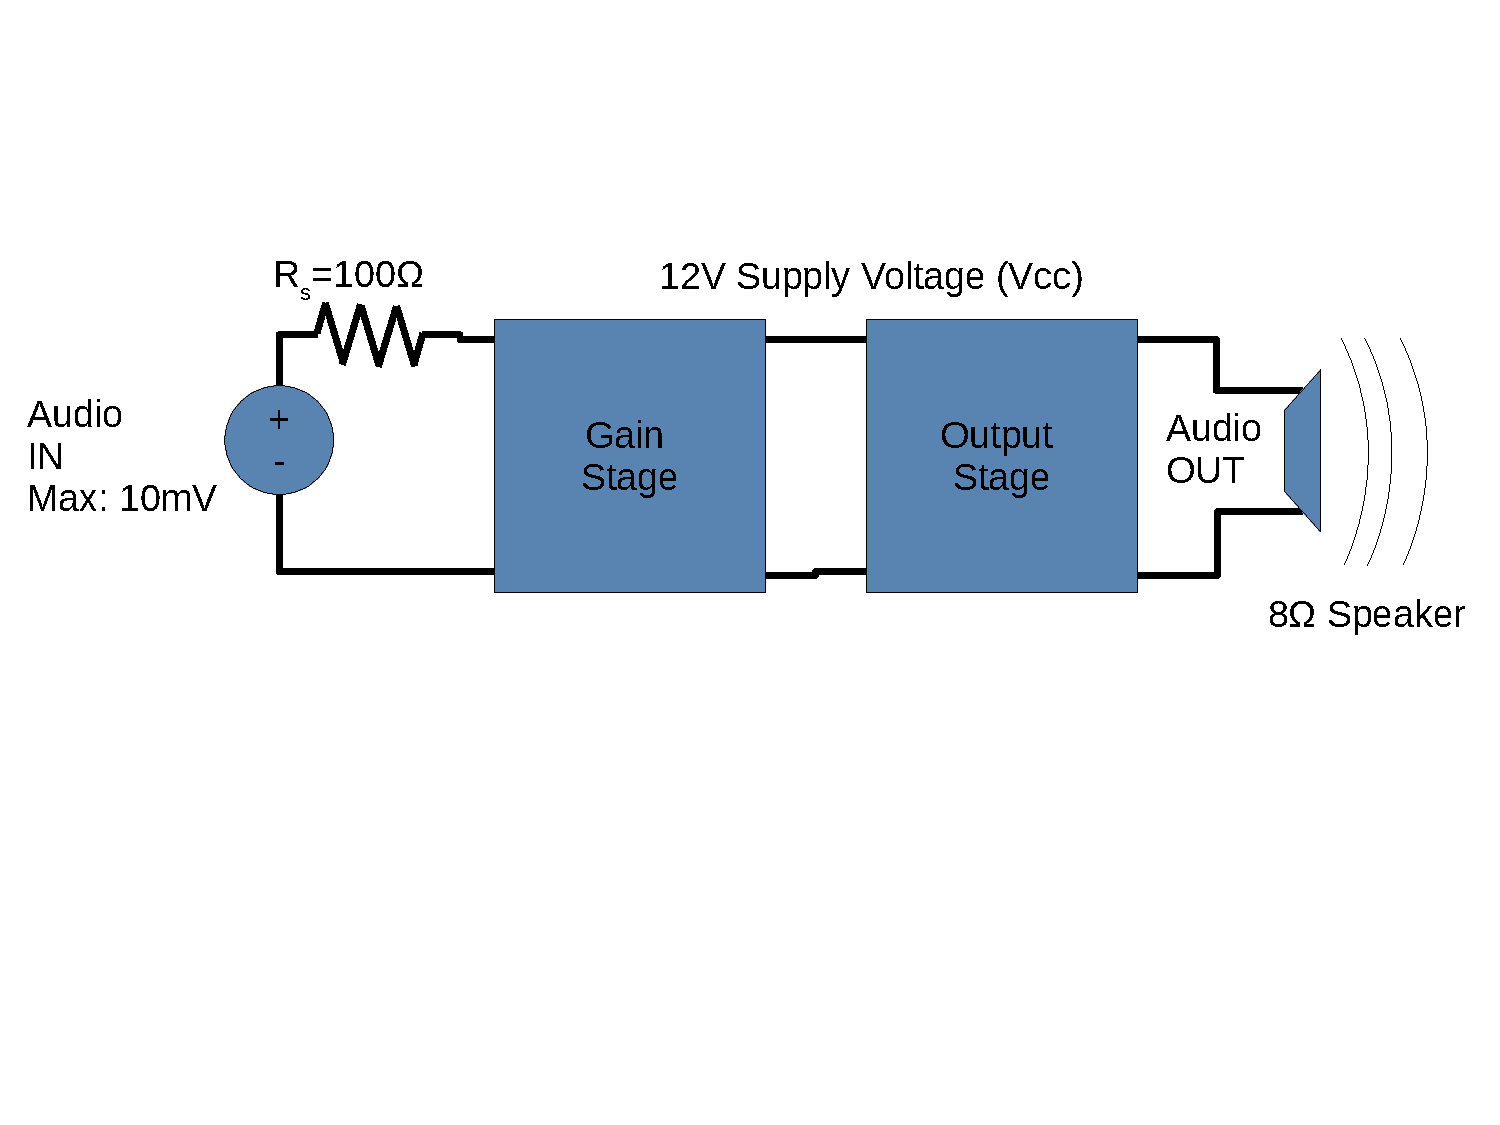
\includegraphics[width=1\linewidth]{circuito.pdf}
\caption{Circuit in analysis}
\label{fig:circuito}
\end{figure}


\newpage

Where:
\begin{center}
\begin{table}[H]
 \centering
  \begin{tabular}{|c|c|}
    \hline    
    {\bf Name} & {\bf Value [A or V]} \\ \hline
    \input{../mat/data_tab}
  \end{tabular}
  \caption{Results obtained by mesh analysis method with octave}
  \label{tab:mesh}
\end{table}
\end{center}

The units of the elements whose name starts with $R$ (the resistors) are $\Omega$ (ohm), $V_s$ is expressed in $V$ (volts) and $C$ is given in $F$ (farad). While $K_b$ is given in $S$ (siemens), $K_c$ is also given in $\Omega$.

These values where obtained using the Python script using the lowest student number on our group - 95785.




\section{Theoretical Analysis}
\label{sec:analysis}

\hspace{0,5cm} In this section, the circuit shown in Figure~\ref{fig:circuito} is analysed theoretically, in terms of its node voltages and mesh currents.

\subsection{Mesh Analysis Method}

\hspace{0,5cm} For this mesh method, circular currents are defined in the counter-clockwise direction and then the circuit is evaluated considering those new currents.

Starting by number the nodes arbitrarily, assigning current names and directions to all branches also arbitrarily and defining one node as ground (GND). 

Being mesh A the one with the resistors $R_1$, $R_3$ and $R_4$, and the voltage source $V_a$, the mesh B with the resistors $R_2$, $R_3$ and $R_5$ and the voltage controlled current source $I_b$, the mesh C with the resistors $R_4$, $R_6$ and $R_7$, and the current controlled voltage source $V_c$, and, at last, the mesh D with the resistor $R_5$, the current source $I_d$ and the current controlled voltage source $V_c$. 

A system of equations obtained applying the Kirchhoff Current Law (KCL)to each mesh can be written as 

\begin{equation}
\begin{bmatrix} 
R_1 + R_3 + R_4 & -R_3 & -R_4 \\ 
-R_4 & 0 & R_4 + R_6 + R_7 - K_C\\
-K_B R_3 & K_B R_3 - 1 & 0
\end{bmatrix} 
\begin{bmatrix} 
I_A \\ 
I_B \\ 
I_C
\end{bmatrix} =
\begin{bmatrix} 
-V_A \\ 
0 \\ 
0
\end{bmatrix}
\end{equation}

It was used 3 equations (4 meshes - 1 = 3 linearly independent equations): Mesh A, Mesh C and an addicional equation which is 

\begin{equation}
I_b = K_b V_b \textit{where} V_b = (I_B - I_A)R_3
\end{equation}

It's important to notice that D loop is independent of the remaining ones so it isn't don't need to determine the current $I_D$ as it is given on the initial data.

Also, mesh B is not used because it has an independent current source so the KVL can't be applied.

After solving the system with Octave tools we get the Table~\ref{tab:mesh} results.

\begin{table}[h]
  \centering
  \begin{tabular}{|l|r|}
    \hline    
    {\bf Name} & {\bf Value [A or V]} \\ \hline
    IA &   -2.440917089113763e-04\\ \hline
IB &   -2.554476012603903e-04\\ \hline
IC &    9.804366878292505e-04\\ \hline
ID &    1.014556835690000e-03\\ \hline
Ib &   -2.554476012603903e-04\\ \hline
Ic &    9.804366878292505e-04\\ \hline
Vb &   -3.572796600675846e-02\\ \hline
Vc &    7.966966194871432e+00\\ \hline

  \end{tabular}
  \caption{ Results obtained by mesh analysis method with octave tool}
  \label{tab:mesh}
\end{table}


\subsection{Nodal Analysis Method}

\hspace{0,5cm} The Nodal Analysis Method is another general procedure for analysing circuits using node voltages as the circuit variables. 

To find the nodal voltages we chose 7 equations (8 nodes - 1 = 7 linearly independent equations) that comprise:
\begin{itemize}
\item  KCL in nodes not connected to voltage sources;
\item Additional equations for nodes related by voltage sources.
\end{itemize}

It was used the equations regarding the nodes 0, 2, 5, 6 therefore it was necessary three additional equations.

We chose to put the ground zero between three branches corresponding to the ones with $R_1, R_2$ and $R_3$ because it will facilitate the system of equations.

The next equation was used for node 1 because node 1 and node 4 are connected to an independent voltage source.
\begin{equation}
V_1-V_4=V_a 
\end{equation}

Secondly knowing that $V_c=K_c I_c$ and $V_c=V_3 - V_7$  it was concluded that for node 7 the equation obtained was $V_3 - V_7 = K_c (V_3 - V_6) G_6$

ATENÇÃO AQUI SFF
Finally, node 3 is connected to 4 branches so applying Ohms Law to the 3 resistors and knowing that the current that passes through $V_c$ is $I_4=-I_d+(V_6-V_7)G_7$ we get the final and third equation that we need: (V4-V3)G4 + (V0-V3)G3 +(V5-V3)G5-Id+(V6-V7)G7=0 %ISTO NAO PODE SER VISTO ASSIM 

The system of equations that will be solved is:


\begin{equation}
\begin{bmatrix} 
1 & 0 & 0 & 0 & 0 & 0 & 0 & 0 \\
-G_1 - G_2 - G_3 & G_1 & G_2 & G_3 & 0 & 0 & 0 & 0 \\
K_b + G_2 & 0 & -G_2 & -K_b & 0 & 0 & 0 & 0 \\
0 & 1 & 0 & 0 & -1 & 0 & 0 & 0 \\
-K_b & 0 & 0 & K_b + G_5 & 0 & -G_5 & 0 & 0 \\
0 & 0 & 0 & 0 & G_6 & 0 & -G_6 - G_7 & G_7 \\
0 & 0 & 0 & 1 & -K_c G_6 & 0 & K_c G_6 & -1 \\
G_3 & 0 & 0 & -G_4 - G_3 - G_5 & G_4 & G_5 & G_7 & -G_7
\end{bmatrix} 
\begin{bmatrix} 
V_0 \\ 
V_1 \\ 
V_2 \\ 
V_3 \\ 
V_4 \\ 
V_5 \\ 
V_6 \\ 
V_7
\end{bmatrix} =
\begin{bmatrix} 
0\\ 
0 \\ 
0 \\ 
V_a \\
-I_d \\ 
0 \\ 
0 \\ 
I_d
\end{bmatrix}
\end{equation}


After solving the system with Octave tools we get the Table~\ref{tab:nodal} results.

\begin{table}[h]
  \centering
  \begin{tabular}{|l|r|}
    \hline    
    {\bf Name} & {\bf Value [A or V]} \\ \hline
    V0 &    0.000000000000000e+00\\ \hline
V1 &    2.524677350223437e-01\\ \hline
V2 &   -5.181833543548797e-01\\ \hline
V3 &    3.572796600675687e-02\\ \hline
V4 &   -4.904491610977656e+00\\ \hline
V5 &    4.000301352954461e+00\\ \hline
V6 &   -6.935136583530766e+00\\ \hline
V7 &   -7.931238228864721e+00\\ \hline
Vb &   -3.572796600675687e-02\\ \hline
Ib &   -2.554476012603790e-04\\ \hline
Vc &    7.966966194871478e+00\\ \hline
Ic &    9.804366878292561e-04\\ \hline

  \end{tabular}
  \caption{Results obtained by nodal analysis method with octave tool}
  \label{tab:nodal}
\end{table}





\section{Simulation Analysis}
\label{sec:simulation}

\subsection{Operating Point Analysis}

Table~\ref{tab:op} shows the simulated operating point results for the circuit
under analysis. Compared to the theoretical analysis results, one notices the
following differences: describe and explain the differences.


\begin{figure}[h] \centering
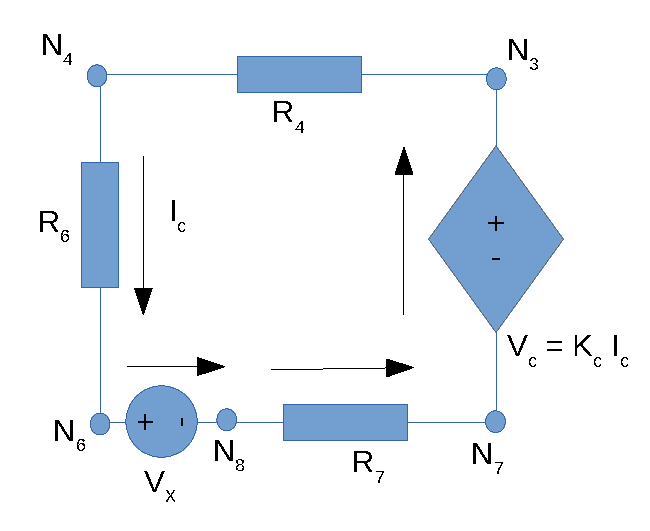
\includegraphics[width=0.4\linewidth]{malhaC.pdf}
\caption{C Mesh with an adicional voltage source} %mudar legendaaaaaaaaaaa!!!!!!
\label{fig:malhaC}
\end{figure}

\begin{table}[h]
  \centering
  \begin{tabular}{|l|r|}
    \hline    
    {\bf Name} & {\bf Value [A or V]} \\ \hline
    @cb[i] & 0.000000e+00\\ \hline
@ce[i] & 0.000000e+00\\ \hline
@q1[ib] & 7.022567e-05\\ \hline
@q1[ic] & 1.404513e-02\\ \hline
@q1[ie] & -1.41154e-02\\ \hline
@q1[is] & 5.765392e-12\\ \hline
@rc[i] & 1.411536e-02\\ \hline
@re[i] & 1.411536e-02\\ \hline
@rf[i] & 7.022567e-05\\ \hline
@rs[i] & 0.000000e+00\\ \hline
v(1) & 0.000000e+00\\ \hline
v(2) & 0.000000e+00\\ \hline
base & 2.254108e+00\\ \hline
coll & 5.765392e+00\\ \hline
emit & 1.411536e+00\\ \hline
vcc & 1.000000e+01\\ \hline

  \end{tabular}
  \caption{Operating point. A variable preceded by @ is of type {\em current}
    and expressed in Ampere; other variables are of type {\it voltage} and expressed in
    Volt.}
  \label{tab:op}
\end{table}

\lipsum[1-1]





%\section{Side by Side Comparison}
\label{sec:comparison}

After ending both simulation and theoretical analysis processes, the results were presented on their sections. However, for presenting a prudent interpretation of the result both tables were put side by side.

\subsection{Envelope detector}

The simulated results of the envelope detector output obtained in NGSpice are compared to the theoretical results from Octave as shown below in Figures \ref{fig:sim41} and \ref{fig:vout_env}, respectively.

\begin{figure} [ht]
\centering
\begin{minipage}{.5\textwidth}
  \centering
  \includegraphics[width=0.9\linewidth]{../sim/sim41.pdf}
  \captionof{figure}{Simulated Envelope detector voltage output}
  \label{fig:sim41}
\end{minipage}%
\begin{minipage}{.5\textwidth}
  \centering
  \includegraphics[width=0.9\linewidth]{vout_env.eps}
  \captionof{figure}{Theoretical Envelope detector voltage output}
  \label{fig:vout_env}
\end{minipage}
\end{figure}

The theoretical ripple in the envelope detector is considerably smaller than the simulated one, due to the approximations made in the theoretical diode model.

\begin{figure}
\centering
\begin{minipage}{.5\textwidth}
  \centering
  \includegraphics[width=0.8\linewidth]{../sim/sim42.pdf}
  \captionof{figure}{Simulated voltage output error.}
  \label{fig:sim_error}
\end{minipage}%
\begin{minipage}{.5\textwidth}
  \centering
  \includegraphics[width=0.8\linewidth]{vout_rect.eps}
  \captionof{figure}{Theoritical voltage output error.}
  \label{fig:theo_error}
\end{minipage}
\end{figure}

\subsection{Output Voltage}
The figures 13 and 14 show the comparison between simulated and theoretical values for the voltage transformer being evident there is no difference between the two plots.
The simulated results of the voltage output are compared to the theoretical results as shown below in Figures \ref{fig:sim_vout} and \ref{fig:theo_vout}, respectively.

\begin{figure} [h]
\centering
\begin{minipage}{.5\textwidth}
  \centering
  \includegraphics[width=0.9\linewidth]{../sim/sim43.pdf}
  \captionof{figure}{Simulated voltage output.}
  \label{fig:sim_vout}
\end{minipage}%
\begin{minipage}{.5\textwidth}
  \centering
  \includegraphics[width=0.9\linewidth]{vout_reg.eps}
  \captionof{figure}{Theoretical voltage output.}
  \label{fig:theo_vout}
\end{minipage}
\end{figure}

Once again, the theoretical ripple is considerably smaller than the simulated one, due to the approximations made in the theoretical diode model.

It is also notable that the theoretical output voltage values are always higher than both 12V and the simulation's values, which are lower than 12V.  

The voltage output errors ($V_{out}$ - 12) of the simulation and the theoretical analysis are shown above in Figures \ref{fig:sim_error} and \ref{fig:theo_error}, respectively.


\begin{figure}
\centering
\begin{minipage}{.5\textwidth}
  \centering
  \includegraphics[width=0.8\linewidth]{../sim/sim44.pdf}
  \captionof{figure}{Simulated voltage output error.}
  \label{fig:sim_error}
\end{minipage}%
\begin{minipage}{.5\textwidth}
  \centering
  \includegraphics[width=0.8\linewidth]{defletion.eps}
  \captionof{figure}{Theoretical voltage output error.}
  \label{fig:theo_error}
\end{minipage}
\end{figure}

\pagebreak The theoretical output voltage error is always positive and higher than the simulation's, which is always negative and bigger in absolute value.
Comparing the Voltage ripple and VDC of the simulated and theoretical analysis in tables \ref{tab:sim} and \ref{tab:tab1}, respectively:

\begin{table}[h]
  \centering
  \begin{tabular}{|l|r|}
    \hline    
    {\bf Name} & {\bf Value [V]} \\ \hline
    \input{../sim/op1_tab}
  \end{tabular}
  \caption{Simulated results. mean(v(4)) is the average outuput voltage and vecmax(v(4))-vecmin(v(4)) is the maximum value of ripple. The last value is the merit of the circuit.}
  
  \label{tab:sim}
\end{table}

\begin{table}[h]
  \centering
  \begin{tabular}{|l|r|}
    \hline    
    {\bf Name} & {\bf Value [V]} \\ \hline
    \input{../mat/octave5_tab}
  \end{tabular}
  \caption{Theoretical values. $V_{DC}$ is the average outuput voltage.}
  \label{tab:tab1}
\end{table}












\newpage
\section{Conclusion}
\label{sec:conclusion}

\hspace{0,5cm} The objective of this laboratory assignment was to develop a Bandpass Filter and the main goal was achieved. 

\par However by observing analysis and simulation results side by side it can be seen a difference between the two, the results aren't equal and exactly the same comparing both NGSpice and Octave. 
\par Although, we believe that the differences are not that significant and they can be explained by how NGSpice solves the circuit compared to how it was done in the theoretical analysis, processes that were also explanied on our lectures. To solve this non-linear circuit, NGSpice used far more advanced simulation methods, with many more parameters, while Octave used an approximated model in incremental analysis. 
\par Regarding this fact and despite the differences, the theoretical model provides good results and can be used when there is no simulation tools to use or to quickly confirmed the simulation results obtained.

\par Nevertheless it was achieved not having the best merit. The merit of the circuit was obtained by trial and error, a method that is not perfect and does not result in the best possible results. In this way, we concluded that in order to obtain good results, we were obliged to "yield" part of the merit.

\par This way, the objective should have never been to have equal results, but rather, have results that seemed reasonables, which we believe it was achieved. The merit obtained was 531.75, with a cost of 1197.5.






%\cleardoublepage

% ----------------------------------------------------------------------
%  Bibliography
% ----------------------------------------------------------------------
%\addcontentsline{toc}{section}{\bibname}
%\bibliographystyle{abbrvunsrtnat} % <<<<< SELECT IF USING REFERENCES BY NUMBER (CITATION ORDER)
%\bibliography{../../../BIBfile.bib}

% ----------------------------------------------------------------------
\end{document}
% ----------------------------------------------------------------------

